% What is MIxT used for? And how would users do it in VR?
% How the MIxT application is implemented in GeneNet VR and what it does.
% What are typical network characteristics for this (type of) application? Size, clusters, edges, connectivity, etc?

\section{What is MIxT used for?}
MIxT blood-tumor is a web application for interactive data exploration in system biology developed by UiT and Concordia University\cite{fjukstad_dumeaux_olsen_lund_hallett_bongo_2017}. In addition, a reasearch was carried out for the study of interactions between the tumor and the blood systemic response of breast cancer patients\cite{dumeaux_fjukstad_interactions_tumor_blood}. In the study, they profiled RNA in blood and matched tumor from 173 patients with breast cancer. The goal of the study was to identify genes and pathways in the primary tumor that are tightly linked to genes and pathways in the patient's systemic response (SR). The SR is the body's response to an infectious or noninfectious insult. A biological pathway is a series of actions among the molecules in a cell that leads to a certain product or change in the cell. The result of the study suggests new ways of monitor breast cancer by looking outside the tumor and studying the patient's systemic response.

Many of the diagnosis for breast cancer are based on a biopsy extracted from the tumor. This will determine the state of the desease and also what treatment to use on the patient. By identifying rekationships between the biopsy and the SR, we can create new ways of diagnosis for this desease.

\begin{figure}[h!]
    \setlength{\tempheight}{15ex}
    \centering
    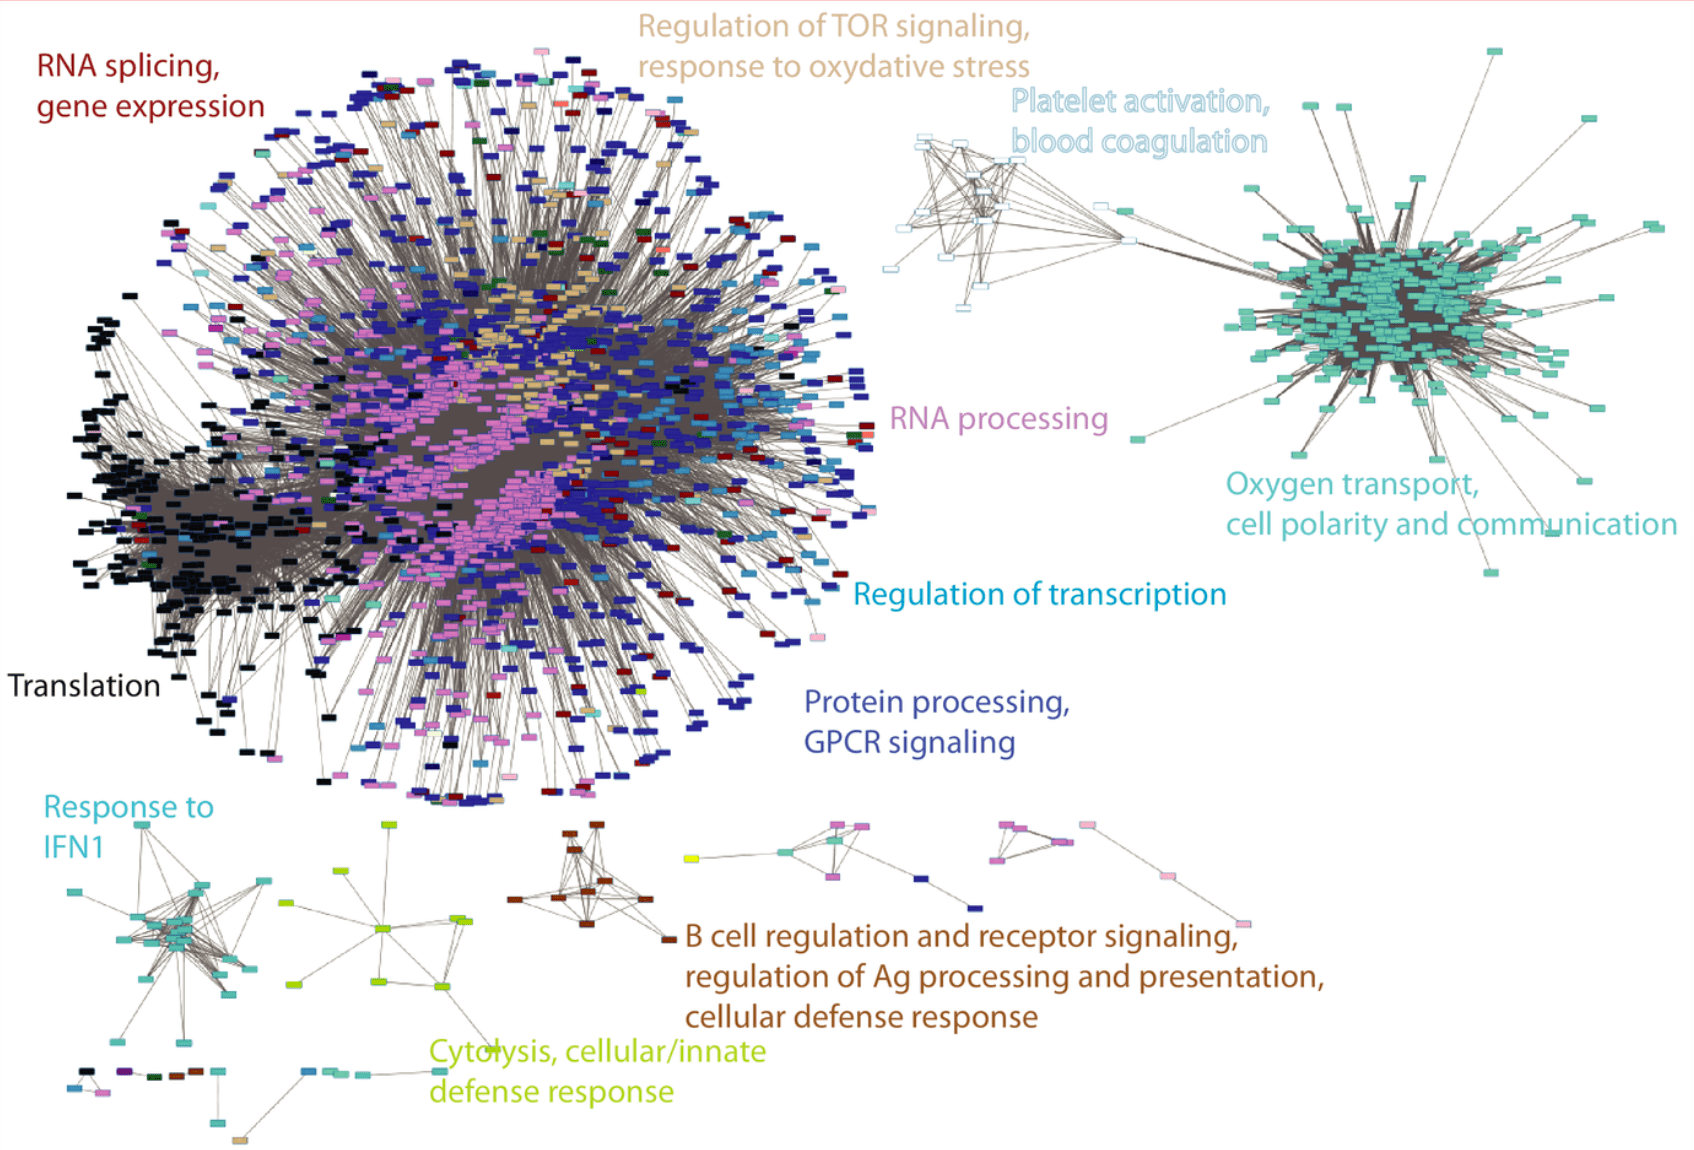
\includegraphics[width=\textwidth]{mixt_paper}
    \caption{Network visualization including the top gene connections in the patient SR. Each node (gene) is color-coded by the module to which it belongs, Keywords representing top pathway enrichments (biological processes) are indicated for each module. Figure from \cite{dumeaux_fjukstad_interactions_tumor_blood}}
    \label{fig:mixt_paper}
\end{figure}

\section{MIxT in VR}

\section{Network characteristics}
